\section{Model Fine Tuning}
\label{model_tuning}
Having trained and evaluated multiple models adjusted with different sets of parameters, it is now time select the best one and fine tune it in order to improve its performances.\\

According to previous testing the best model for this particular task is the Naive Bayes Classifier. With a ROC AUC score of 0.6 it managed to achieve an average precision of 1\% and a fairly high average recall of 60\% all be it with a little bit of deviation between runs (Figure \ref{nbc_d}).\\

Using a grid search method \cite{grid_scikit} it is possible to find the best combination of parameters for a classifier. The Gaussian classifier from de Scikit-Learn library unfortunatly has only one. Still, performing a grid search on this parameter which correspond to the portion of the largest variance of all features that is added to variances for calculation stability \cite{nbc_scikit}. Testing a hundred value evenly spaced on a log scale between \(1\) and \(10^{-15}\) and using the ROC AUC score, it found that a value close to \(10^{-7}\) is the best choice for the \textit{var\_smoothing} parameter.\\

Nevertheless, the results did not improve at all if not deteriorate. The avrage ROC AUC score still hovers around 60\%, the average precision looks similar but the average recall droped form 59\% to 53\% meaning the model is not as good at finding defective items on the production line.

\begin{figure}
    \center
    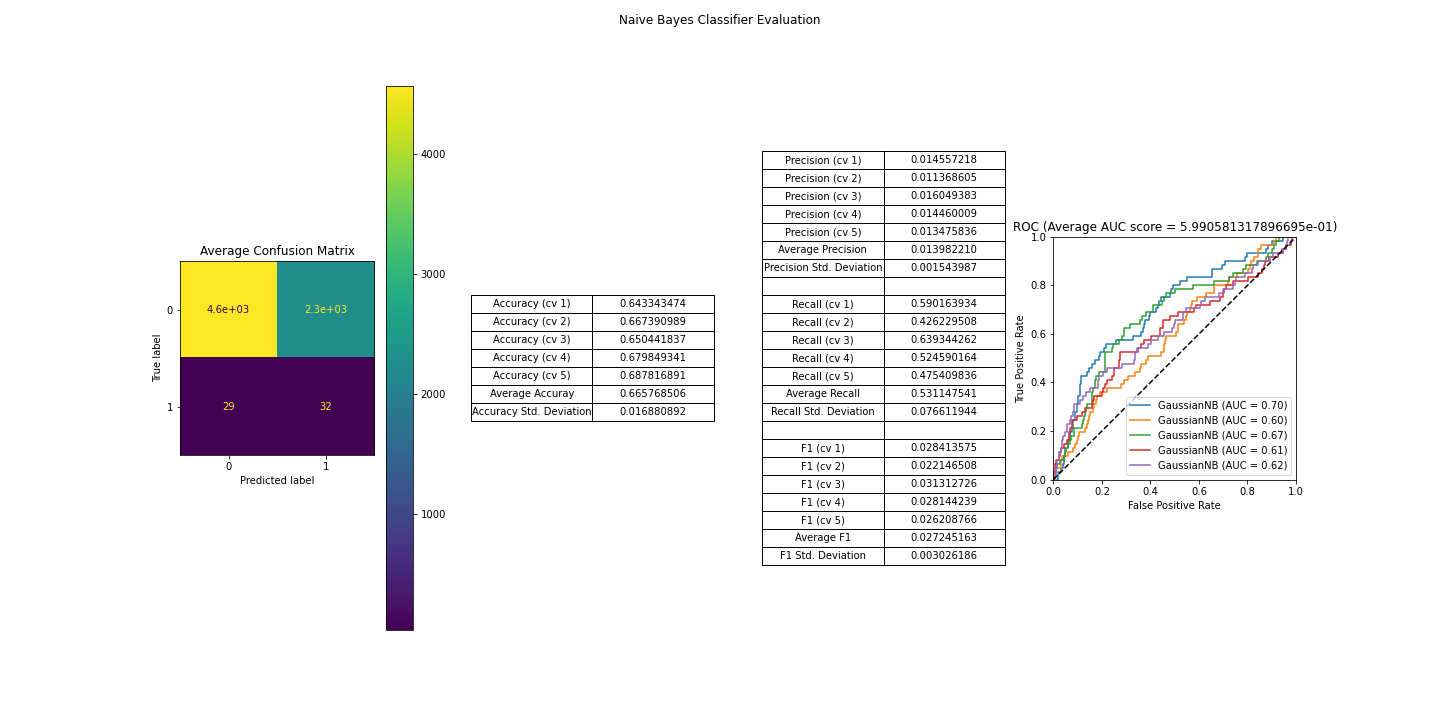
\includegraphics[scale=0.32]{img/nbc_gd.png}
    \caption{Naive Bayes Classifier Evaluation with tuned parameters}
    \label{nbc}
\end{figure}